\documentclass{exam}

\usepackage{Haust2016verkefnablöð}

\title{Stærðfræðimynstur í tölvunarfræði \\ Skilaverkefni 8}
\author{}

\printanswers

\begin{document}
\maketitle
\thispagestyle{empty} 

Skila skal þessu verkefni á vefnum \href{https://gradescope.com/}{Gradescope}. Aðgangskóði fyrir námskeiðið er \textbf{926WD9}.


\section{Spurningar}

\begin{questions}

\section{Kafli 9.1}

\question Útskýrið hvort eftirfarandi vensl á mengi rauntalnanna séu sjálfhverf, samhverf, andsamhverf og/eða gegnvirk, þar sem $(x, y)$ er í venslunum þá og því aðeins að
\begin{enumerate}[a)]
 \item $x = 2y$
 \item $xy \geq 0$
\end{enumerate}

\paragraph{Í bók} Hluti af exercise 9.1.6

\question Látum $R$ vera vensl frá mengi $A$ til mengis $B$. Þá getum við skilgreint andhverfu venslin $R^{-1} = \{(b, a) | (a, b) \in R\}$ sem eru frá $B$ til $A$. Við getum líka skilgreint fyllivenslin $\overline{R} = \{(a, b) | (a, b) \notin R\}$.

Skoðum nú venslin $R = \{(a, b) | a < b\}$. Hvað er

\begin{enumerate}[a)]
 \item $R^{-1}$?
 \item $\overline{R}$?
\end{enumerate}

\paragraph{Í bók} Exercise 9.1.26

\section{Kafli 9.2}

\question Sýnið að ef $C$ er skilyrði sem $n$-undir í $n$-undarvenslunum $R$ og $S$ geta uppfyllt, þá sé
\[s_C(R \cup S) = s_C(R)\cup s_C(S)\]

\paragraph{Í bók} Exercise 9.2.20
\newpage
\question Gefin er eftirfarandi tafla:
\begin{center}
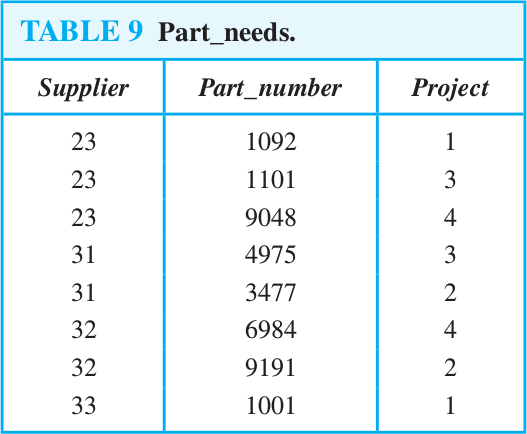
\includegraphics[width=0.6\textwidth]{parts-table}
\end{center}
ásamt eftirfarandi SQL-skipun sem vinnur á töflunni:
\begin{minted}[frame=lines]{sql}
SELECT Supplier
FROM Part_needs
WHERE 1000 <= Part_number AND Part_number <= 5000
\end{minted}
Svo er spurt:

\begin{enumerate}[a)]
 \item Hvaða virkjar koma við sögu í þessari SQL-skipun og hvaða áhrif hefur hver þeirra á niðurstöðuna?
 \item Hver er niðurstaða þessarar SQL-skipunar?
\end{enumerate}

\paragraph{Í bók} Exercise 9.2.28

\section{Kafli 9.3}

\question Látum $R$ vera vensl á $n$ staka mengi. Séu $k$ ásar í fylkinu $M_R$ sem táknar $R$, hversu margir ásar eru í fylkinu $M_{R^{-1}}$ sem táknar andhverfu venslin $R^{-1}$? Rökstyðjið niðurstöðuna.

\paragraph{Í bók} Exercise 9.3.16
\newpage
\question
\begin{enumerate}[a)]
 \item Teiknaðu stefnt net fyrir venslin $\{(a, a), (a, b), (b, c), (c, b), (c, d), (d, a), (d, b)\}$.
 \item Teldu upp röðuðu pörin í venslunum sem eftirfarandi stefnt net skilgreinir:
\end{enumerate}
\begin{center}
 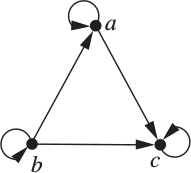
\includegraphics[width=0.33\textwidth]{triangle-graph}
\end{center}
\paragraph{Í bók} Exercise 9.3.22 og 9.3.24
\end{questions}


\end{document}